\begin{figure}[ht]
\centering
% Thesis-wide categorical color palette
% Usage: % Thesis-wide categorical color palette
% Usage: % Thesis-wide categorical color palette
% Usage: \input{figures/palette} in any figure file
%
% Muted primary colors -- print-friendly, visually distinct.
% Inspired by Cooper Union's red/blue primaries, softened for
% academic figures. Use palA-palC for data series in scatter
% plots, line charts, bar charts, etc.

\definecolor{palA}{HTML}{1F77B4}   % Tableau blue
\definecolor{palB}{HTML}{D62728}   % Tableau red
\definecolor{palC}{HTML}{2CA02C}   % Tableau green
 in any figure file
%
% Muted primary colors -- print-friendly, visually distinct.
% Inspired by Cooper Union's red/blue primaries, softened for
% academic figures. Use palA-palC for data series in scatter
% plots, line charts, bar charts, etc.

\definecolor{palA}{HTML}{1F77B4}   % Tableau blue
\definecolor{palB}{HTML}{D62728}   % Tableau red
\definecolor{palC}{HTML}{2CA02C}   % Tableau green
 in any figure file
%
% Muted primary colors -- print-friendly, visually distinct.
% Inspired by Cooper Union's red/blue primaries, softened for
% academic figures. Use palA-palC for data series in scatter
% plots, line charts, bar charts, etc.

\definecolor{palA}{HTML}{1F77B4}   % Tableau blue
\definecolor{palB}{HTML}{D62728}   % Tableau red
\definecolor{palC}{HTML}{2CA02C}   % Tableau green

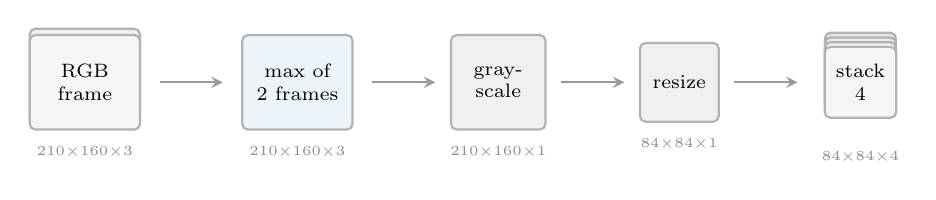
\begin{tikzpicture}[
    box/.style={draw=black!30, thick, minimum height=1.2cm,
                font=\scriptsize, inner sep=4pt, align=center,
                rounded corners=2pt},
    arr/.style={->, thick, >=stealth, black!40},
    dimlbl/.style={font=\tiny, text=black!45},
]

% Raw frames (two overlapping)
\node[box, minimum width=1.4cm, fill=black!6]
    (raw2) at (0, 0.08) {};
\node[box, minimum width=1.4cm, fill=black!4]
    (raw1) at (0, 0) {RGB\\frame};
\node[dimlbl, below=2pt] at (raw1.south)
    {210${\times}$160${\times}$3};

\draw[arr] (0.95, 0) -- (1.75, 0);

% Max of two frames
\node[box, minimum width=1.4cm, fill=palA!8]
    (maxf) at (2.7, 0) {max of\\2 frames};
\node[dimlbl, below=2pt] at (maxf.south)
    {210${\times}$160${\times}$3};

\draw[arr] (3.65, 0) -- (4.45, 0);

% Grayscale
\node[box, minimum width=1.2cm, fill=black!6]
    (gray) at (5.25, 0) {gray-\\scale};
\node[dimlbl, below=2pt] at (gray.south)
    {210${\times}$160${\times}$1};

\draw[arr] (6.05, 0) -- (6.85, 0);

% Resize
\node[box, minimum width=1.0cm, minimum height=1.0cm,
      fill=black!6]
    (resize) at (7.55, 0) {resize};
\node[dimlbl, below=2pt] at (resize.south)
    {84${\times}$84${\times}$1};

\draw[arr] (8.25, 0) -- (9.05, 0);

% Stack 4 frames (four overlapping boxes)
\node[box, minimum width=0.9cm, minimum height=0.9cm,
      fill=black!10] at (9.85, 0.18) {};
\node[box, minimum width=0.9cm, minimum height=0.9cm,
      fill=black!8] at (9.85, 0.12) {};
\node[box, minimum width=0.9cm, minimum height=0.9cm,
      fill=black!6] at (9.85, 0.06) {};
\node[box, minimum width=0.9cm, minimum height=0.9cm,
      fill=black!4]
    (stack) at (9.85, 0) {stack\\4};
\node[dimlbl, below=8pt] at (stack.south)
    {84${\times}$84${\times}$4};

\end{tikzpicture}
\caption{Preprocessing pipeline. Two consecutive raw frames are
  combined, converted to grayscale, resized, and stacked to produce
  the input tensor for the network.}
\label{fig:preprocessing}
\end{figure}
